\chapter{A Grand Apparatus}
\begin{aquote}{Fran\c{c}ois Englert, CMS: The Art of Science, 2016}
    A glance at the ATLAS and CMS detectors at CERN reveals their beauty...
    These detectors are the modern cathedrals of the rational world created by scientists, experimentalists, and theoreticians. 
\end{aquote}
\section{The Large Hadron Collider}
% Give some history
%    - collider physics + others? (i.e. ...so we bury enormous colliders underground, still others position enormous film cameras to...)
%    - Some pictures of groundbreaking?
%    - LEP?
%    - Some impressive plots/pictures (e.g. arial shot, of course)
\section{The Compact Muon Solenoid}
\begin{figure}[htb]
    \centering
    \includegraphics[width=0.9\textwidth]{fig/cms/cms_labeled.jpg}
    \caption{
        Lorem ipsum.
    }
    \label{fig:cms_labeled}
\end{figure}
\subsection{Superconducting solenoid}
\subsection{Silicon tracker}
\subsection{Electromagnetic calorimeter}
\subsection{Hadronic calorimeter}
\subsection{Muon chambers}
% Overview: "Compact" "Muon" "Solenoid"?
%    - i.e. what is it supposed to do?
%    - show diagram from UChicago proposal of the generalized particle layers
% Explain each layer
%    - mention russia shells --> calorimeter
\begin{figure}[htb]
    \centering
    \subfloat{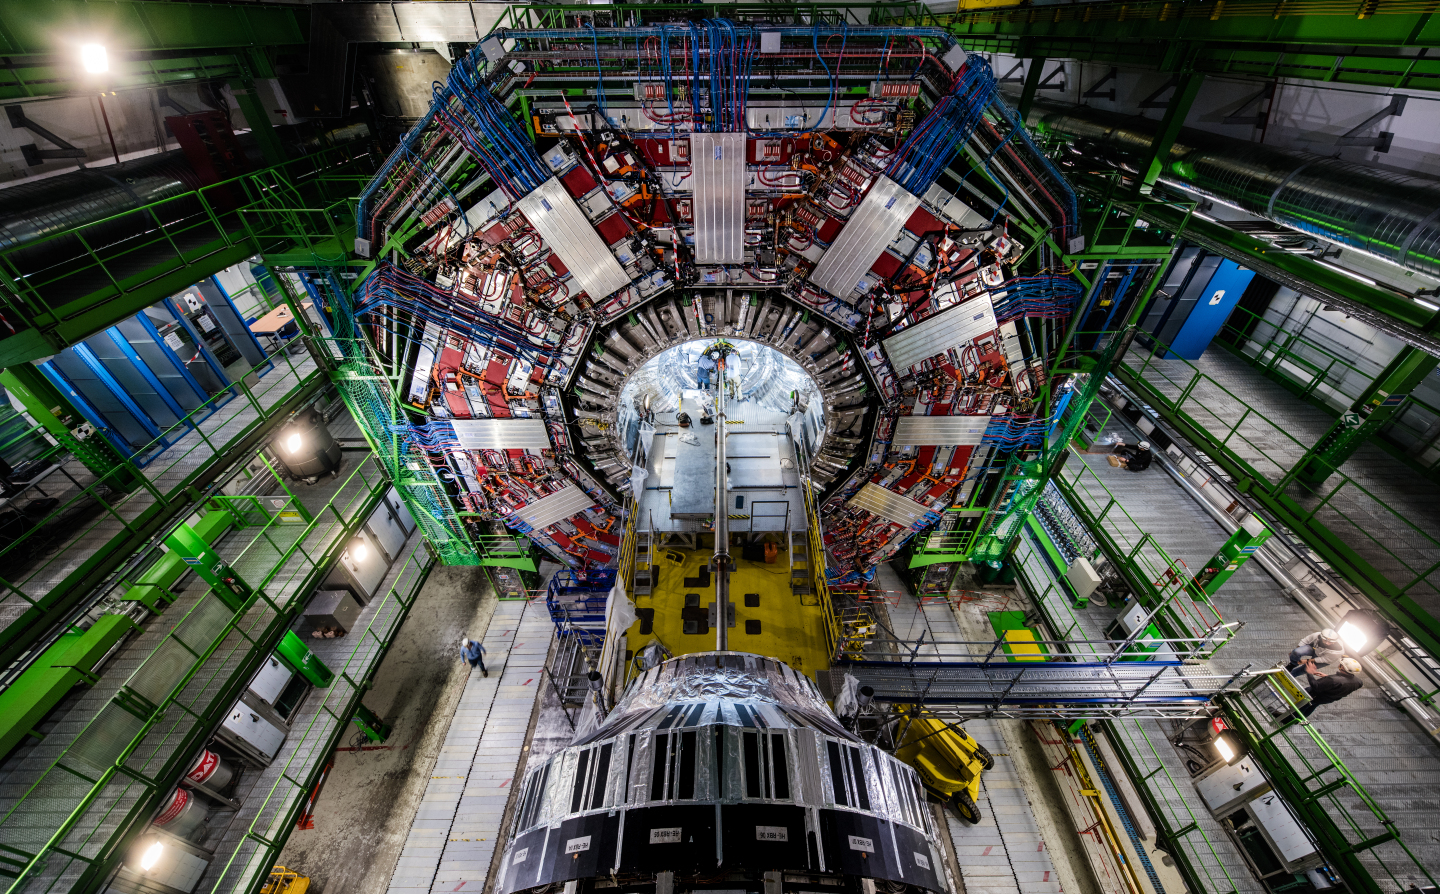
\includegraphics[width=0.465\textwidth]{fig/cms/cms_picture1.jpg}}\quad
    \subfloat{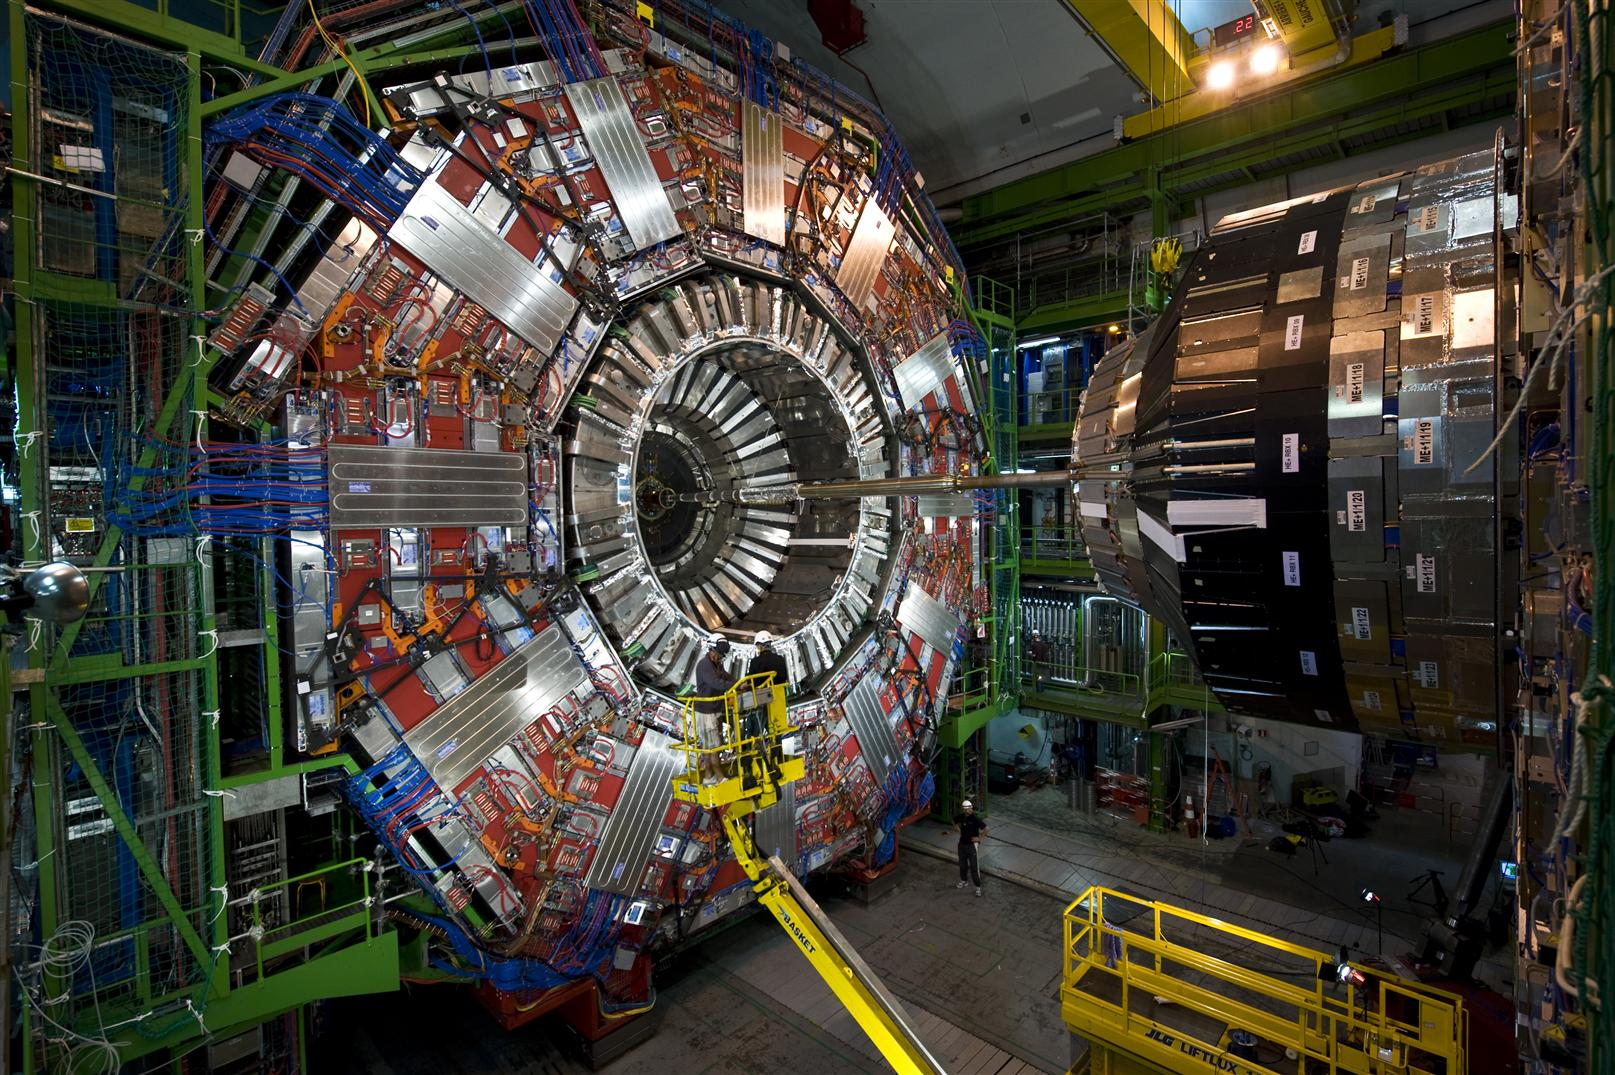
\includegraphics[width=0.435\textwidth]{fig/cms/cms_picture2.jpg}}
    \caption{
        lorem ipsum.
    }
    \label{fig:cms_pics}
\end{figure}

\begin{figure}[htb]
    \centering
    \subfloat{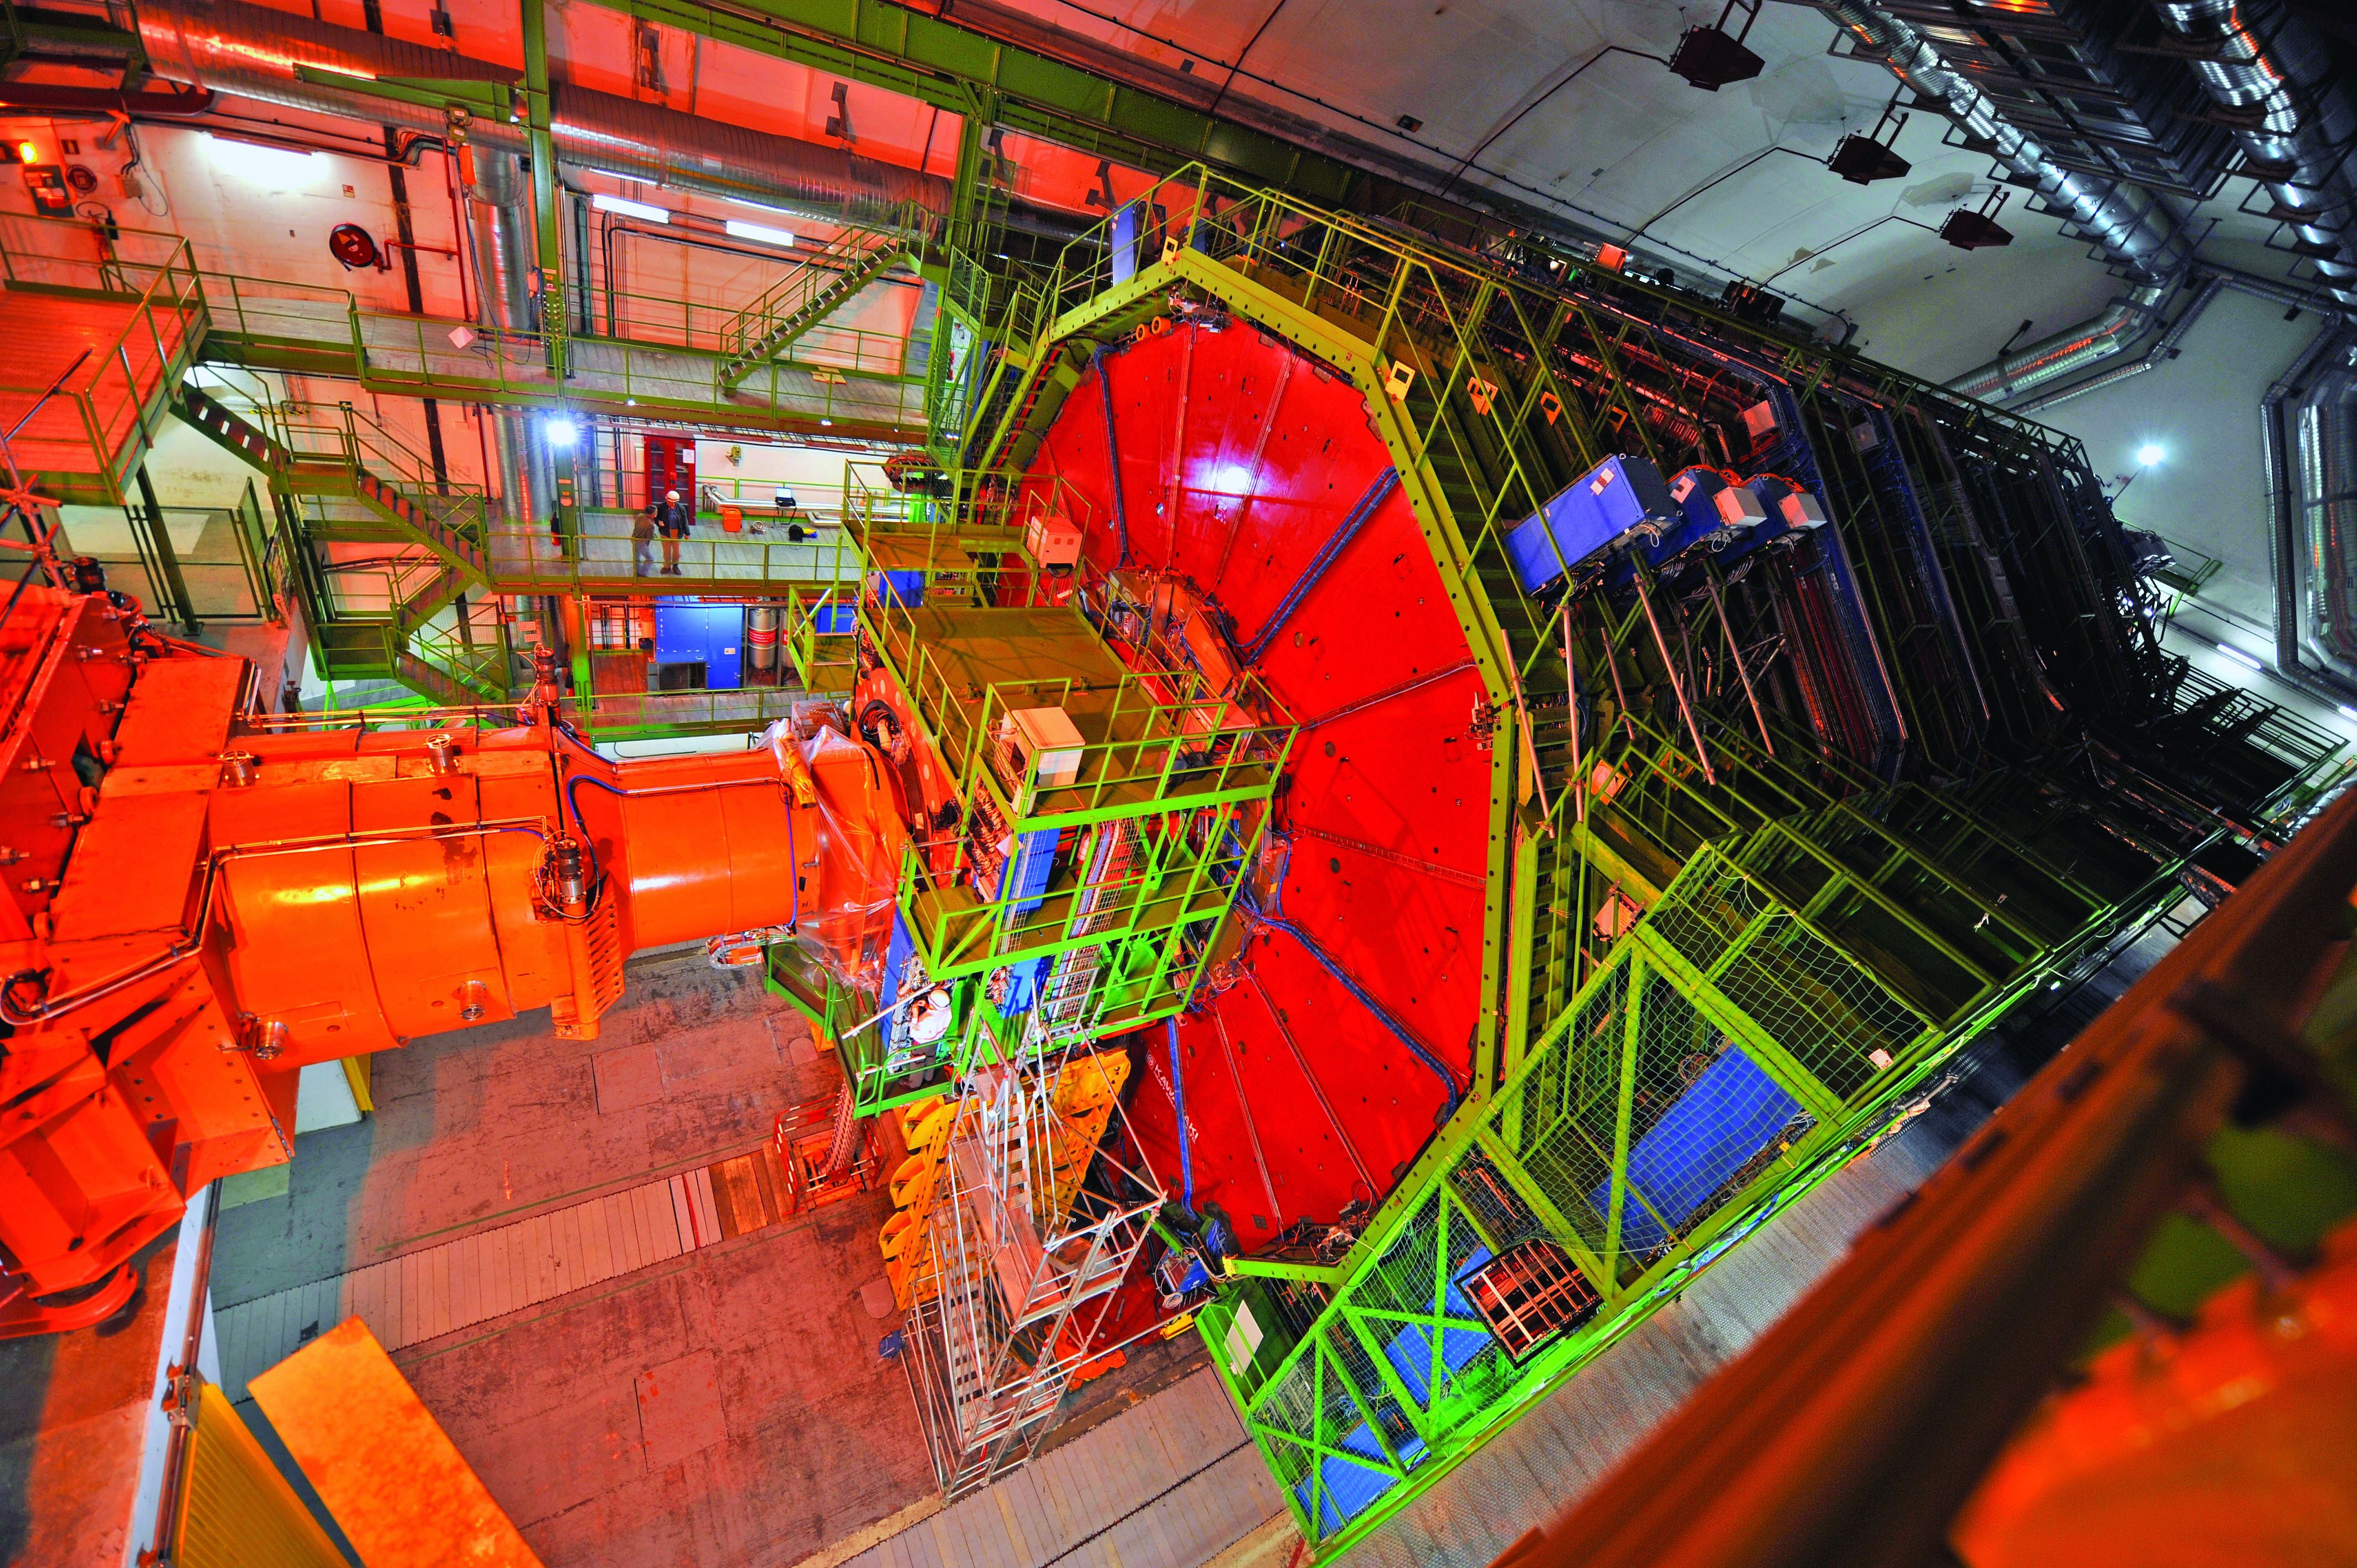
\includegraphics[width=0.482\textwidth]{fig/cms/cms_picture3.jpg}}\quad
    \subfloat{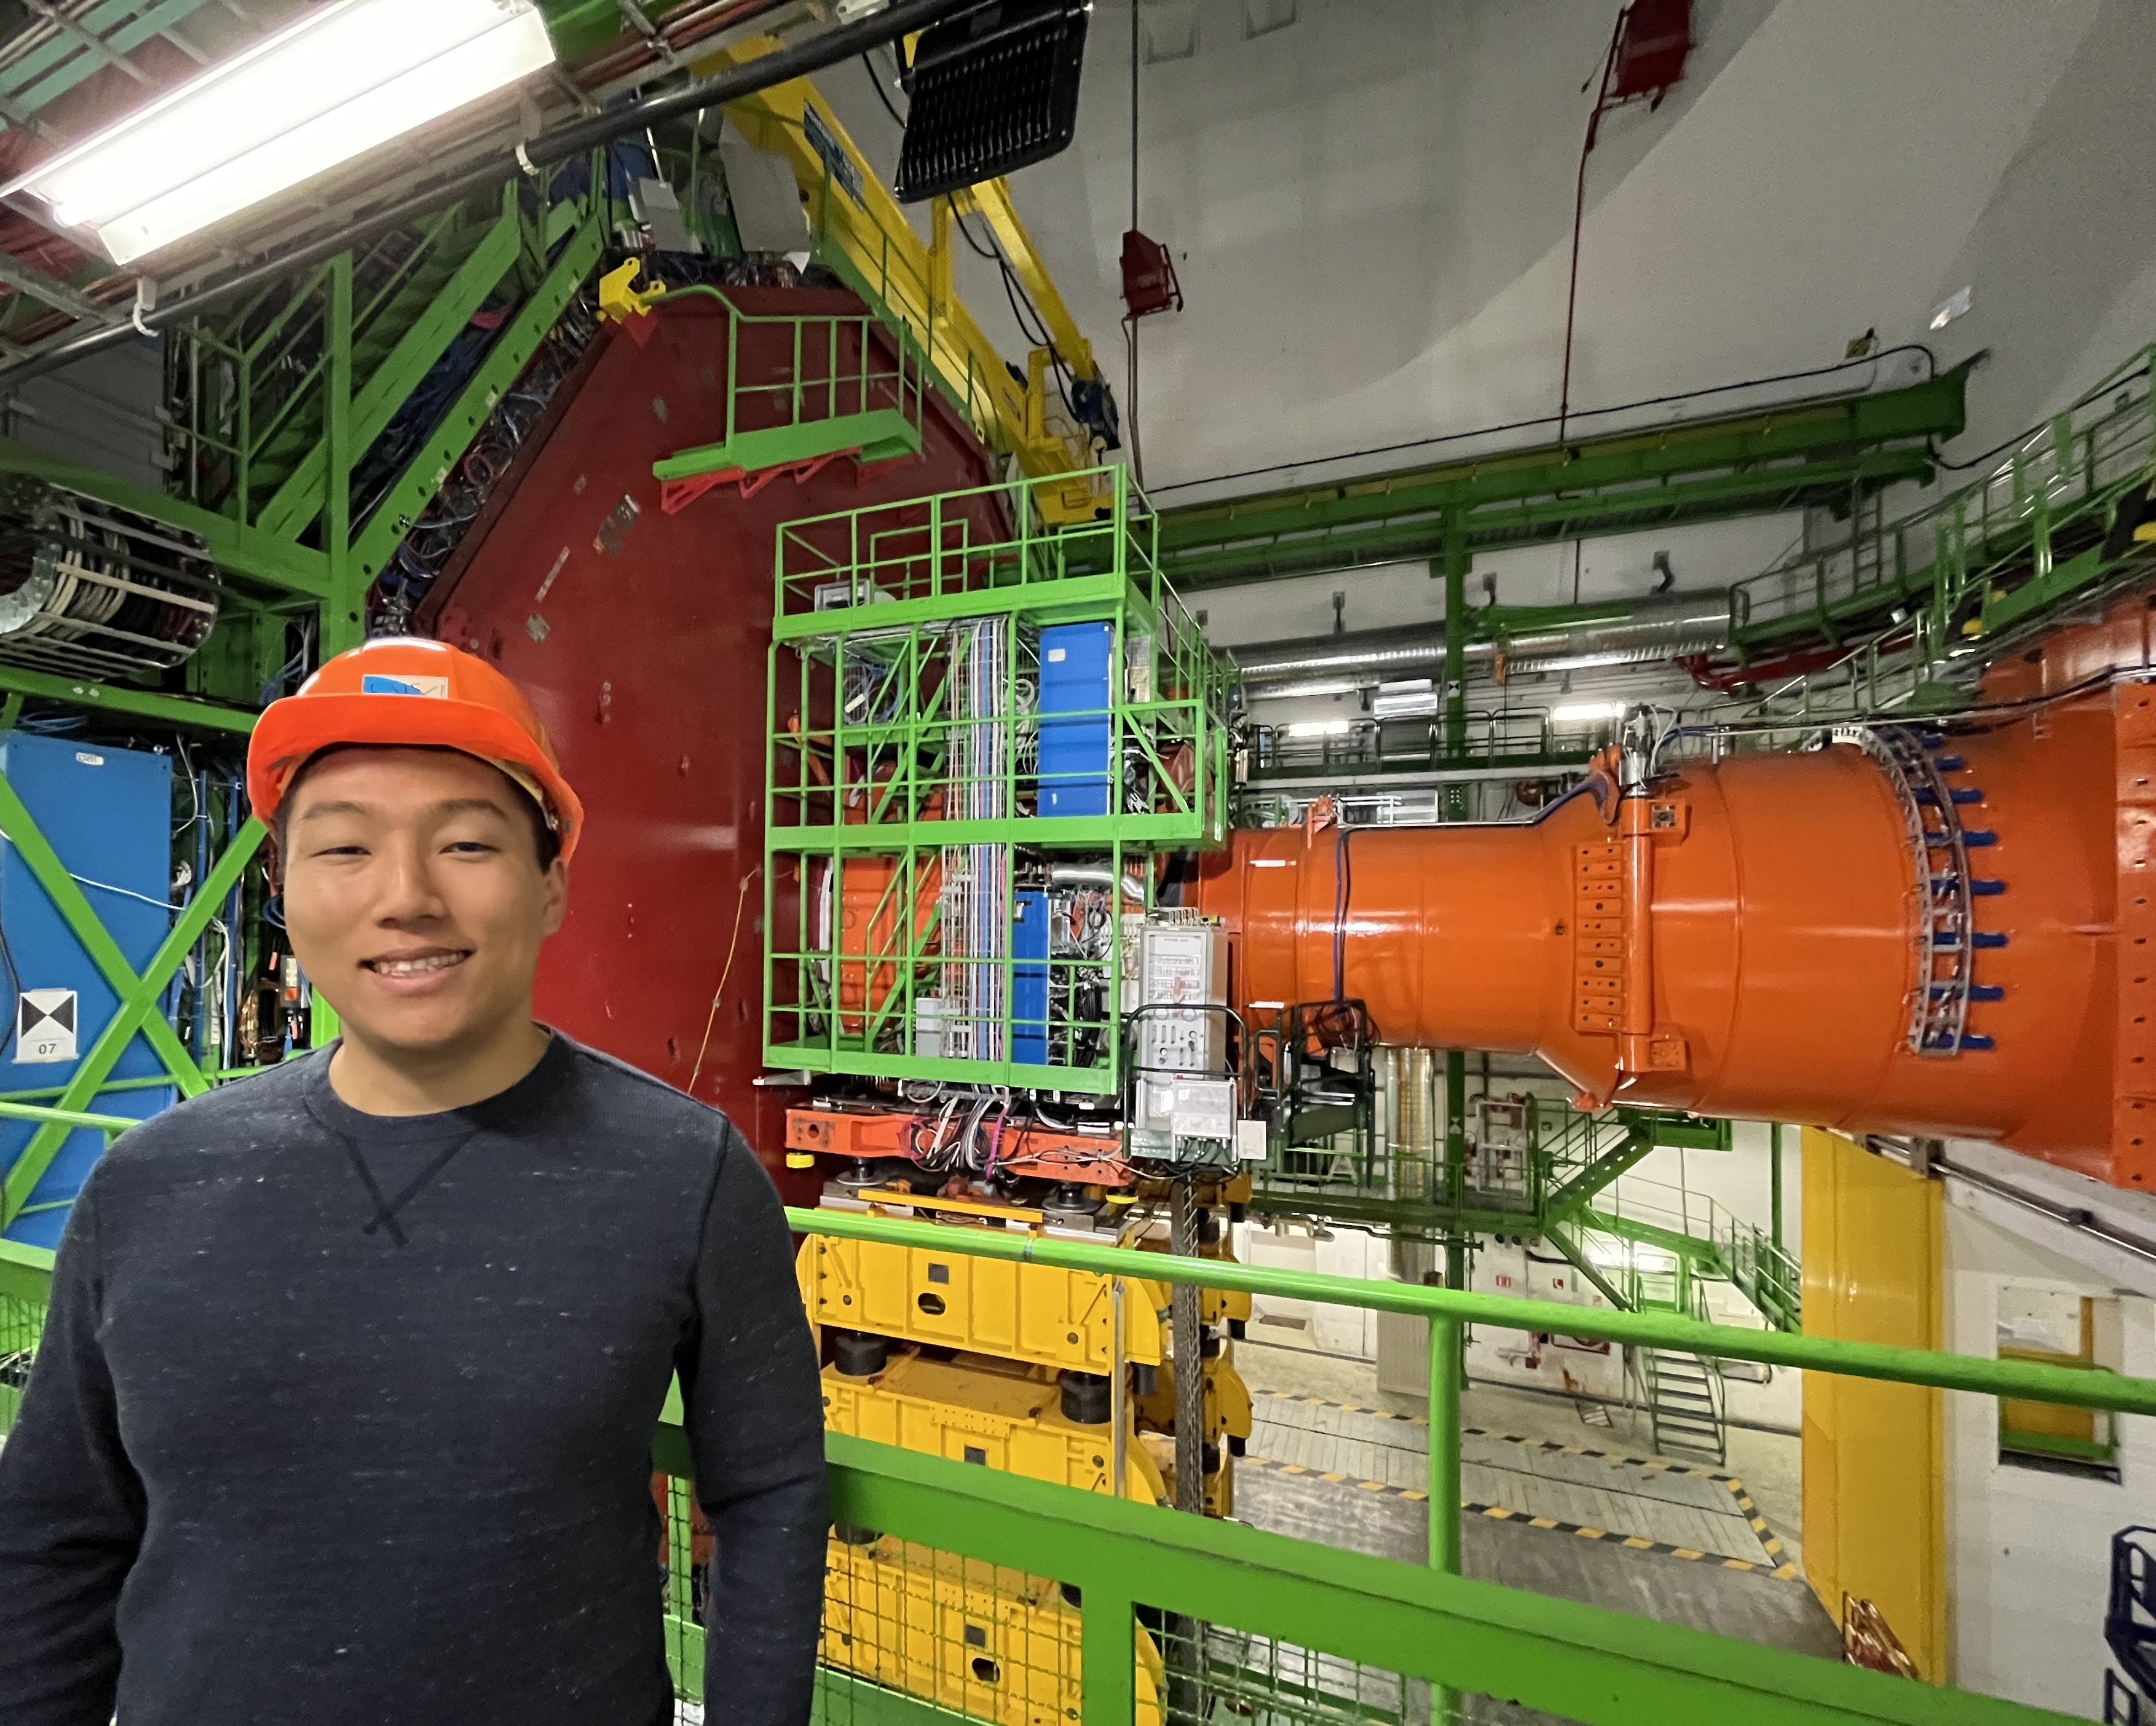
\includegraphics[width=0.4\textwidth]{fig/cms/cms_jguiang.jpg}}
    \caption{
        Lorem ipsum.
    }
    \label{fig:cms_jguiang}
\end{figure}
\section{The high lumonisity era}
% What is HL?
%    - show pileup plots, maybe side AND 3D volume
% What benefits does it bring?
%    - Find some papers...
% What challenges does it bring?
%    - Show CPU/Data volume plots
